\newif\ifshowsolutions
\showsolutionstrue
\documentclass{article}
\usepackage{listings}
\usepackage{amsmath}
%\usepackage{subfigure}
\usepackage{subfig}
\usepackage{amsthm}
\usepackage{amsmath}
\usepackage{amssymb}
\usepackage{graphicx}
\usepackage{mdwlist}
\usepackage[colorlinks=true]{hyperref}
\usepackage{geometry}
\usepackage{titlesec}
\geometry{margin=1in}
\geometry{headheight=2in}
\geometry{top=2in}
\usepackage{palatino}
\usepackage{mathrsfs}
\usepackage{fancyhdr}
\usepackage{paralist}
\usepackage{todonotes}
\setlength{\marginparwidth}{2.15cm}
\usepackage{tikz}
\usetikzlibrary{positioning,shapes,backgrounds}
\usepackage{float} % Place figures where you ACTUALLY want it
\usepackage{comment} % a hack to toggle sections
\usepackage{ifthen}
\usepackage{mdframed}
\usepackage{verbatim}
\usepackage[strings]{underscore}
\usepackage{listings}
\usepackage{bbm}
\rhead{}
\lhead{}

\renewcommand{\baselinestretch}{1.15}

% Shortcuts for commonly used operators
\newcommand{\E}{\mathbb{E}}
\newcommand{\Var}{\operatorname{Var}}
\newcommand{\Cov}{\operatorname{Cov}}
\newcommand{\Bias}{\operatorname{Bias}}
\DeclareMathOperator{\argmin}{arg\,min}
\DeclareMathOperator{\argmax}{arg\,max}

% do not number subsection and below
\setcounter{secnumdepth}{1}

% custom format subsection
\titleformat*{\subsection}{\large\bfseries}

% set up the \question shortcut
\newcounter{question}[section]
\newenvironment{question}[1][]
  {\refstepcounter{question}\par\addvspace{1em}\textbf{Question~\Alph{question}\!
    \ifthenelse{\equal{#1}{}}{}{ [#1 points]}: }}
    {\par\vspace{\baselineskip}}

\newcounter{subquestion}[question]
\newenvironment{subquestion}[1][]
  {\refstepcounter{subquestion}\par\medskip\textbf{\roman{subquestion}.\!
    \ifthenelse{\equal{#1}{}}{}{ [#1 points]:}} }
  {\par\addvspace{\baselineskip}}

\titlespacing\section{0pt}{12pt plus 2pt minus 2pt}{0pt plus 2pt minus 2pt}
\titlespacing\subsection{0pt}{12pt plus 4pt minus 2pt}{0pt plus 2pt minus 2pt}
\titlespacing\subsubsection{0pt}{12pt plus 4pt minus 2pt}{0pt plus 2pt minus 2pt}


\newenvironment{hint}[1][]
  {\begin{em}\textbf{Hint: }}{\end{em}}

\ifshowsolutions
  \newenvironment{solution}[1][]
    {\par\medskip \begin{mdframed}\textbf{Solution~\Alph{question}#1:} \begin{em}}
    {\end{em}\medskip\end{mdframed}\medskip}
  \newenvironment{subsolution}[1][]
    {\par\medskip \begin{mdframed}\textbf{Solution~\Alph{question}#1.\roman{subquestion}:} \begin{em}}
    {\end{em}\medskip\end{mdframed}\medskip}
\else
  \excludecomment{solution}
  \excludecomment{subsolution}
\fi



%%%%%%%%%%%%%%%%%%%%%%%%%%%%%%
% HEADER
%%%%%%%%%%%%%%%%%%%%%%%%%%%%%%

\chead{
  {\vbox{
      \vspace{2mm}
      \large
      Machine Learning \& Data Mining \hfill
      Caltech CS/CNS/EE 155 \hfill \\[1pt]
      Miniproject 1\hfill
      February 2019. \\
    }
  }
}

\begin{document}
\pagestyle{fancy}



%%%%%%%%%%%%%%%%%%%%%%%%%%%%%%
% PROBLEM 1
%%%%%%%%%%%%%%%%%%%%%%%%%%%%%%

\newpage

\section{Introduction [20 points]}

\vspace{2ex}

\noindent
Group members: Maria De Angelis, Tanvi Gupta, Ziyan Mo

\noindent
Github: https://github.com/maria93101/cs155-kaggle

\noindent
Team name: BirbML

\noindent
2008 private leaderboard ranking: 36

\noindent
2012 private leaderboard ranking: 23

\noindent
2008 private leaderboard AUC score: 0.79171
\
\noindent
2012 private leaderboard AUC score: 0.78384

\noindent
Division of labor:
\begin{itemize}
\item Tanvi: Data cleanup, neural networks
\item Ziyan: Data export, decision trees, XGBoost, SVM, k-means, merging data from different methods
\item Maria: Random forests, SVM, merging data from different methods
\end{itemize}

\newpage

\section{Overview [20 points]}

\vspace{2ex}

\noindent
\textbf{Models and Techniques}

\noindent
We tried multiple different models in order to explore which ones would work best on a regression problem, since we’ve usually dealt with classification in class. The first of these was a neural network, for which we tried between 1 and 3 dense layers with activations and dropouts. Another thing that we tried at the very beginning was decision trees and (eventually) random forests regressions. After taking a look at the data, we noticed some branching conditions which would work well with these models, and so we attempted to enhance them with gradient boosting (specifically, XGBoost). 

\noindent
For each of our models, we used some of the techniques discussed in class to prevent under- or over-fitting; this included setting an appropriate ratio of units and layers for the neural net, testing different stopping conditions for decision trees/random forests, and even attempting an “average” of all of our models to get a less skewed output.

\noindent
Some models which we considered initially but discarded were K-means, SVM, and AdaBoost, because of their unsuitability for regression problems.

\vspace{1ex}
\noindent
\textbf{Timeline}

\noindent
We started investigating the data on Friday and figuring out what columns to clean up. On Saturday to Monday, we each investigated our own models. On Monday, we looked at the best submissions to the  public board on kaggle, and decided to try and merge the best public models -- XGboost and neural net. Tuesday was spent trying to improve the 2 best models and merging other lesser models. 

\newpage

\section{Approach [20 points]}

\vspace{2ex}

\noindent
\textbf{Data Processing and Manipulation}

\noindent
Studying the training data as well as the provided codebook revealed that since the parameters are actually survey questions, there were some (ex. HRHHID - the respondent’s unique ID) that weren’t relevant to the model at all. There were also a few columns which had only one response type for all the datapoints (ex. HRMONTH - the month in which this survey was conducted). We discarded these columns, since they just create extra noise from our models and detract from the weight given to the other features. A lot of this analysis was done using Excel’s filter commands.

\noindent
Since all the data was numeric, we also took the opportunity to normalize it to [0,1] in order to be more easily processed by the neural network models. We used Scikit-Learn’s preprocessing tools library (MinMaxScaler) for the normalization. This seemed to work quite well, but another option to explore would be one-hot-encoding the features, which might further simplify the processing in a neural network.

\noindent
We also did some post-processing of the output, mainly to ensure that it met the criteria for being a physically possible probability of voting. A small fraction of the neural network and XGBoosting results were less than zero or greater than one. We tried two approaches to remedy this. The first was to normalize the predicted values to be between zero and one (using MinMaxScaler), which, while solving the issue, does have the unintended consequence of pushing the rest of the output values closer together (the overall range of possibilities is decreased). The second was to simply re-assign any values lower than zero to zero, and any values greater than one to one. If a predicted value is higher or lower than the boundaries, it likely just means that the algorithm is more certain that a voter will or will not vote. Thus, we can simply assign 0/1, without having to tamper with the less certain probabilities.

\vspace{1ex}
\noindent
\textbf{Model and Technique Details}

\begin{enumerate}
\item Neural networks: We decided to start out with a simple neural network, since we know already neural networks are powerful mechanisms for classification problems. We decided to tweak our implementation and explore different layers to suitably adapt the network to a regression problem. Clearly, since this is not an image processing problem, convolution layers would not be very helpful, so we went back to a Dense-layered model, with ReLU activation. We were curious whether the zero-value-ignoring nature of ReLU would affect the regression problem, and so tried a sigmoid activation at first, but ReLU appeared to perform better. In addition, we did not use a Softmax layer at the end, since each individual output should be a probability. We tested two “extremes” - one dense layer with 13 units, and 3 dense layers with 400, 250, and 350 units (with some dropouts in between), and found that the simpler model had a perceptibly better performance. We then built up this model, increasing the number of units until performance seemed to plateau. At this point, we decided to try out other models as well (discussed below). Neural networks are advantageous because they can easily be used to model non-linear and complex relationships, which is very useful with a dataset like ours which has over 300 features. They are adept at generalizing to the data, and slightly less likely to overfit than the other models. A disadvantage of neural networks in this scenario is that they are more useful for classification tasks - theoretically, decision trees would be better for regression.

\item Decision trees and random forests: From the data, we felt that decision trees and random forests are better for this data because of certain branching conditions (such as employment related question), since there are some people who left these questions blank and other questions conditioned on it. Thus, we started off investigating Scikit’s decision trees with default parameters. After some initial testing with cross-validation and looking at the results from Kaggle’s public leaderboard, we decided to investigate further with Scikit’s random forests and fine tuning the parameters. With decision trees, because we have a singular tree, the model is very simplistic (although it did reasonably well). The advantage is what we mentioned as the rationale of using a decision tree -- it intuitively fits how the dataset itself branches. With random forests, some disadvantages are that it is slow in predicting (because there are so many steps) and it is prone to overfitting. Some advantages are that it can be grown in parallel if need (although we did not do it) and it is a very versatile model. 

\item XGBoost: Based on the initial promising result from random forest, we looked more other tree-related models. One package that came up was XGboost, which stands for extreme gradient boosting. They use decision tree ensembles, which seem to be the great given our prior results with random forests. In gradient boosting, many models are created to predict the error of the previous models using the gradient descent algorithm and updating our predictions based on learning rate, and then they are combined by assigning some weight to each one. One advantage of this method is that it is more precise than decision trees and is very fast. One disadvantage is that it is not easily parallelizable because XGBoost needs to use the previous models in order to improve upon the next model (by minimizing the residuals).

\item AdaBoost, SVM, and K-Means: We briefly tried out SVM, Adaboost, and k-means. With SVM, we only tried the linear kernel -- this was obviously a bad choice for this non-linear dataset. The algorithm never converged for obvious reasons. In general SVMs are better for simple classification problems. With k-means, we tried with many centers (10000). However, since that again more classification based, the results were quite bad when we scored it with cross validation. The advantages for k-means are that it is good for finding relations between unlabeled data, but k means clustering is very bad for high dimensional data like what we have here. Adaboost also didn’t improve the performance of our model, giving us an accuracy just above chance. Adaboost is sensitive to outlier and label noise (which we had a lot of since we didn’t do extensive feature selection) which could explain its poor performance on this dataset.
\end{enumerate}

\newpage

\section{Model Selection [20 points]}

\vspace{2ex}

\noindent
\textbf{Scoring}

\noindent
Since we’re performing regression, the built-in metric we used for most of our models was mean squared error, which we used as a quick-glance, baseline test to ensure that the model actually made sense (i.e. MSE wasn’t egregiously large), and to compare models on a high level. For more detailed comparisons (such as how many units to use, what stopping conditions to set), we also consulted the AUC scores, which we computed using Scikit-Learn’s roc_auc_score function in the Metrics package. The AUC score was helpful in giving us a general sense (accounting, of course, for overfitting) of where our models would land on the leaderboard.

\vspace{1ex}
\noindent
\textbf{Validation and Testing}

\noindent
We used a couple of different validation/comparison techniques to contrast our models and pick the best one. We tried to prevent both overfitting and underfitting - trying models against the Kaggle test set was a good way of pinpointing these. The neural-network tests were more of trial-and-error to see how many layers/units gave the best results. For decision trees and random forests, we optimized the hyperparameters for our model by running a simplifying version of  each model with different parameter values. In particular, we found that keeping maximum depth relatively low (around 7) worked well to prevent overfitting. For xgboost, we didn’t do much testing with the parameters since we ran out of time, so we used the parameters from their tutorial.

\noindent
To compute some “shadow” metrics with the training data we were given and to further prevent overfitting, we also used Scikit-Learn’s cross validation methods on our training dataset. For the neural net models, we decided on K=10, i.e. 90\% of the dataset was training and 10\% was validation, and this was repeated 10 times. For the decision tree/random forest models, we decided on K=5, i.e. 20\% of the dataset was validation. This helped us compute more accurate AUC scores of the training y-values versus the predicted training targets, which in turn allowed us to better judge which models might be good for the test dataset.

\noindent
After investigating the many models we noted above, we found that gradient boosting (specifically, XGBoost), and neural networks resulted in the highest area under the curve accuracy. We decided to merge the 2 models’ outputs  to generalize more and further prevent overfitting. We were pleased to note that this approach seemed to work well, since this was our best-performing model on the 2012 dataset.

\newpage~
\newpage

\section{Conclusion [20 points]}

\vspace{2ex}

\noindent
\textbf{Important Features}

\noindent
We used Scikit-Learn’s feature selection library (method SelectKBest), with the f_regression statistical test, to select the 10 most important features. We found that columns (indexed from 0) 6 (HETENURE, money status of living quarters), 41 (PEAGE, a person’s age at survey week), 43 (PEMARTIL, a person’s marital status), 44 (PESPOUSE, line number of spouse), 48 (PEEDUCA, a person’s highest education degree), 57 (PRMARSTA, the marital status of a non-civilian), 237 (PESCHENR, if the person was in secondary or advanced degrees last week), 332 (PXSCHLVL, an allocation flag), 335 (PEDIPGED, how a person got their HS diploma), 338 (PEGRPROF, if the person has completed college classes for credit after college graduation) were the most highly correlated.

\noindent
In addition, the following heatmap shows the correlation between these features and their correlation with the target value. We see that PEAGE, PESPOUSE, PEEDUCA, and PEGRPROF have negative correlation with target (=1), and the other six have positive correlation. Since target=1 corresponds to a person who did not vote, PEAGE, PESPOUSE, PEEDUCA, and PEGRPROF are positively correlated with a person’s likelihood of voting. These observations make sense, since past data has shown that young people vote less. Marital status and high levels of education have also been shown to correspond to a higher voter turnout. We also found that cost of living arrangement is positively correlated with voter participation (high HETENURE is correlated with low voter turnout). This makes sense because people who are not paying for their housing are likely to have unstable living environments and a lower income (those with a lower income have been shown to vote less due to long work hours, and are also less likely to be highly educated). Similarly, the other observations seem to follow expected patterns of voter turnout based on prior knowledge.

\vspace{-2ex}

\begin{figure}[hbt!]
\center
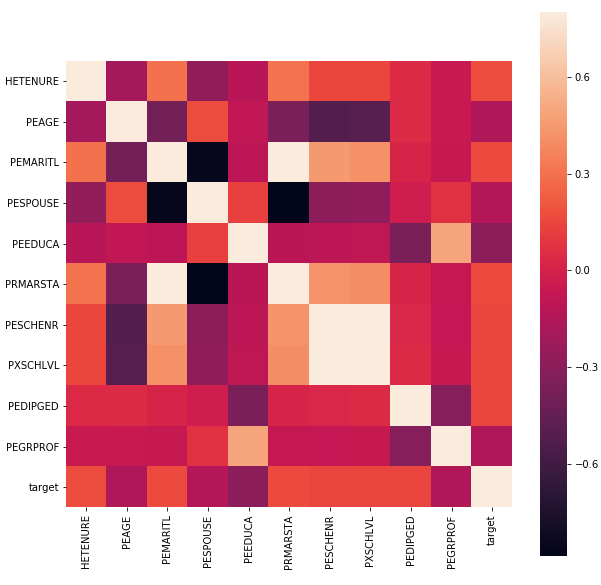
\includegraphics[scale=0.3]{final.png}
\end{figure}

\vspace{-2ex}

\vspace{1ex}
\noindent
\textbf{AUC}

\noindent
The AUC has less false positives and is overall more precise than other metrics we have used such as accuracy. It is useful in cases where it’s important to not have false positives (sometimes at the cost of true positive), such as when deciding if a patient should have an expensive and dangerous surgery. Voter turnout is obviously less critical, but it is better to underestimate voter turnout rather than overestimate it, because historical analysis suggests that voters change their mind and decide not to vote more often than the other way around. For this reason, we think AUC is an appropriate measure for this project.

\vspace{1ex}
\noindent
\textbf{Parallelization}

\noindent
The main models we used - neural nets and random forest can be parallelized. With random forest, since it is a collection of decision trees, no decision depends on the results from another. Because XGBoost needs to use the previous models in order to improve upon the next model (by minimizing the residuals) it is not a good candidate for running on multiple cores.

\vspace{1ex}
\noindent
\textbf{Takeaways}

\noindent
The homeworks so far have had very clear objectives and have had answers that were clearly outlined in the lectures. This project allowed us to work with a raw dataset and a less well defined problem. In doing so, we understood concepts such as data normalization and feature cleanup better. We also got the chance to compare and contrast multiple different models on the same dataset without a prior expectation of which one would perform the best. This definitely mirrors the real-life machine learning process more closely than our problem sets, where we study one topic a week. The open-ended approach to this project helped us in preparation for hands-on projects in the future.

\noindent
In addition, we have mostly worked with linearly separable datasets and classification problems in class, so this project gave us the opportunity to explore different learning models that work well for non- linearly separable, regression datasets. It was an interesting exercise trying to extrapolate from our previous knowledge how things would work in this new problem space.
This project also solidified the concept that sometimes simpler is better! For the neural net model, we tried a variety of models of different complexities, spanning from 10 to 400 nodes in densely connected layers and we found that a simple model actually performed best (overfitted the least).

\vspace{1ex}
\noindent
\textbf{Challenges}

\noindent
If we were to repeat this process, we would spend more time looking at the codebook to get a better understanding of what features are most important to train on. Unfortunately, the codebook was not very easy to parse through, so we were limited in the amount of analysis we were able to do in the time frame, since we decided to focus on trying out many different models. As mentioned in a previous section, we would also try out more initial data processing, such as one-hot-encoding the features for better results on the neural net models.

\noindent
The very cursory “average results” method we employed to combat overfitting worked surprisingly well, and so if given the chance in the future, we would also like to explore ensemble methods and more rigorous ways of combining different models together.

\noindent
Logistically, we could have also split up the work in a more organized fashion. We started by all training our own models and then discussing what worked and what didn’t. While this was helpful in all of us gaining an understanding of the different models, this caused some valuable information to be lost and also prevented us from trying many different types of models (for example, all three of us trained our own neural network when the time could have been better spent exploring different approaches). We abandoned SVM pretty early after seeing bad results, but we could have investigated it further with a ‘poly’ kernel.


\end{document}
